\documentclass{standalone}
\usepackage{tikz}
\usetikzlibrary{patterns, positioning}


\begin{document}
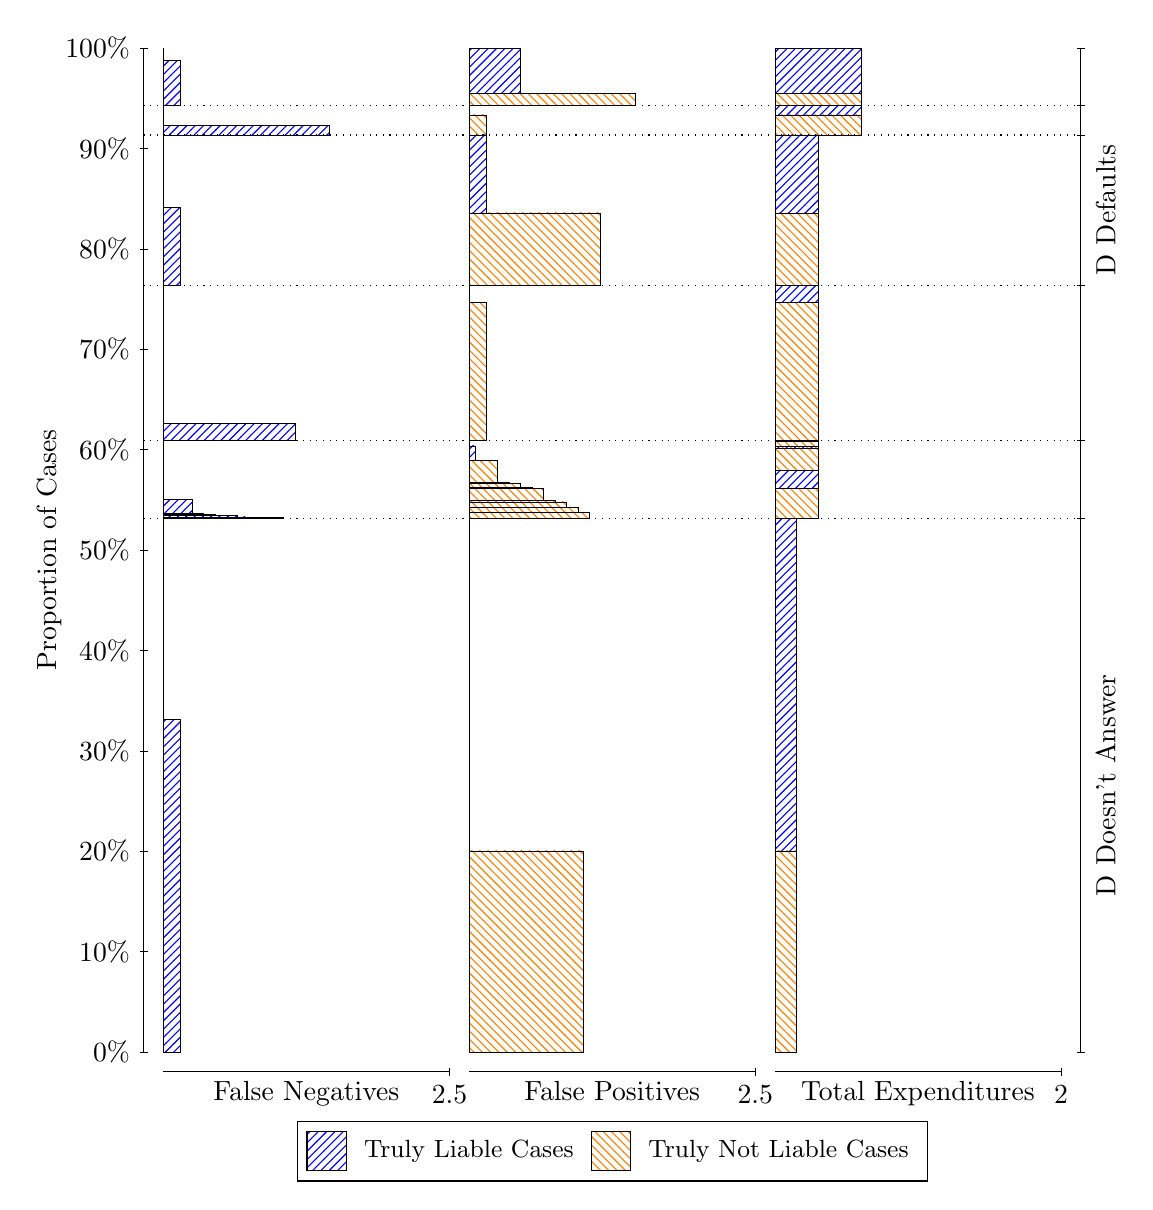
\begin{tikzpicture}
\draw[black, very thin] (1.5,1.75) -- (1.5,14.5);
\node[rotate=90, text=black, anchor=center] at (0.3, 8.125) {Proportion of Cases};
\draw[black, very thin] (1.45,1.75) -- (1.55,1.75);
\node[text=black, anchor=east] at (1.45, 1.75) {0\%};
\draw[black, very thin] (1.45,3.025) -- (1.55,3.025);
\node[text=black, anchor=east] at (1.45, 3.025) {10\%};
\draw[black, very thin] (1.45,4.3) -- (1.55,4.3);
\node[text=black, anchor=east] at (1.45, 4.3) {20\%};
\draw[black, very thin] (1.45,5.575) -- (1.55,5.575);
\node[text=black, anchor=east] at (1.45, 5.575) {30\%};
\draw[black, very thin] (1.45,6.85) -- (1.55,6.85);
\node[text=black, anchor=east] at (1.45, 6.85) {40\%};
\draw[black, very thin] (1.45,8.125) -- (1.55,8.125);
\node[text=black, anchor=east] at (1.45, 8.125) {50\%};
\draw[black, very thin] (1.45,9.4) -- (1.55,9.4);
\node[text=black, anchor=east] at (1.45, 9.4) {60\%};
\draw[black, very thin] (1.45,10.675) -- (1.55,10.675);
\node[text=black, anchor=east] at (1.45, 10.675) {70\%};
\draw[black, very thin] (1.45,11.95) -- (1.55,11.95);
\node[text=black, anchor=east] at (1.45, 11.95) {80\%};
\draw[black, very thin] (1.45,13.225) -- (1.55,13.225);
\node[text=black, anchor=east] at (1.45, 13.225) {90\%};
\draw[black, very thin] (1.45,14.5) -- (1.55,14.5);
\node[text=black, anchor=east] at (1.45, 14.5) {100\%};

\draw[black, very thin] (13.4,1.75) -- (13.4,14.5);
\draw[black, very thin] (13.35,1.75) -- (13.45,1.75);
\node[anchor=west] at (13.35, 1.75) {};
\draw[black, very thin] (13.35,8.5235) -- (13.45,8.5235);
\node[anchor=west] at (13.35, 8.5235) {};
\draw[black, very thin] (13.35,9.5135) -- (13.45,9.5135);
\node[anchor=west] at (13.35, 9.5135) {};
\draw[black, very thin] (13.35,11.489) -- (13.45,11.489);
\node[anchor=west] at (13.35, 11.489) {};
\draw[black, very thin] (13.35,13.396) -- (13.45,13.396);
\node[anchor=west] at (13.35, 13.396) {};
\draw[black, very thin] (13.35,13.769) -- (13.45,13.769);
\node[anchor=west] at (13.35, 13.769) {};
\draw[black, very thin] (13.35,14.5) -- (13.45,14.5);
\node[anchor=west] at (13.35, 14.5) {};

\draw[black, very thin, pattern color=blue, pattern=north east lines] (1.75,1.75) rectangle (1.968,5.9697);
\draw[black, very thin, pattern color=orange, pattern=north west lines] (1.75,5.9697) rectangle (1.75,8.5235);
\draw[black, very thin, pattern color=blue, pattern=north east lines] (1.75,8.5235) rectangle (3.276,8.5402);
\draw[black, very thin, pattern color=blue, pattern=north east lines] (1.75,8.5402) rectangle (3.1307,8.5411);
\draw[black, very thin, pattern color=blue, pattern=north east lines] (1.75,8.5411) rectangle (2.9853,8.5441);
\draw[black, very thin, pattern color=blue, pattern=north east lines] (1.75,8.5441) rectangle (2.84,8.5448);
\draw[black, very thin, pattern color=blue, pattern=north east lines] (1.75,8.5448) rectangle (2.6947,8.5643);
\draw[black, very thin, pattern color=blue, pattern=north east lines] (1.75,8.5643) rectangle (2.5493,8.5676);
\draw[black, very thin, pattern color=blue, pattern=north east lines] (1.75,8.5676) rectangle (2.404,8.5793);
\draw[black, very thin, pattern color=blue, pattern=north east lines] (1.75,8.5793) rectangle (2.2587,8.5895);
\draw[black, very thin, pattern color=blue, pattern=north east lines] (1.75,8.5895) rectangle (2.1133,8.7695);
\draw[black, very thin, pattern color=orange, pattern=north west lines] (1.75,8.7695) rectangle (1.75,9.5135);
\draw[black, very thin, pattern color=blue, pattern=north east lines] (1.75,9.5135) rectangle (3.4213,9.7368);
\draw[black, very thin, pattern color=orange, pattern=north west lines] (1.75,9.7368) rectangle (1.75,11.489);
\draw[black, very thin, pattern color=blue, pattern=north east lines] (1.75,11.489) rectangle (1.968,12.48);
\draw[black, very thin, pattern color=orange, pattern=north west lines] (1.75,12.48) rectangle (1.75,13.396);
\draw[black, very thin, pattern color=blue, pattern=north east lines] (1.75,13.396) rectangle (3.8573,13.515);
\draw[black, very thin, pattern color=orange, pattern=north west lines] (1.75,13.515) rectangle (1.75,13.769);
\draw[black, very thin, pattern color=blue, pattern=north east lines] (1.75,13.769) rectangle (1.968,14.345);
\draw[black, very thin, pattern color=orange, pattern=north west lines] (1.75,14.345) rectangle (1.75,14.5);
\draw[black, very thin, pattern color=orange, pattern=north west lines] (5.6333,1.75) rectangle (7.0867,4.3038);
\draw[black, very thin, pattern color=blue, pattern=north east lines] (5.6333,4.3038) rectangle (5.6333,8.5235);
\draw[black, very thin, pattern color=orange, pattern=north west lines] (5.6333,8.5235) rectangle (7.1593,8.5987);
\draw[black, very thin, pattern color=orange, pattern=north west lines] (5.6333,8.5987) rectangle (7.014,8.6625);
\draw[black, very thin, pattern color=orange, pattern=north west lines] (5.6333,8.6625) rectangle (6.8687,8.7368);
\draw[black, very thin, pattern color=orange, pattern=north west lines] (5.6333,8.7368) rectangle (6.7233,8.7583);
\draw[black, very thin, pattern color=orange, pattern=north west lines] (5.6333,8.7583) rectangle (6.578,8.9062);
\draw[black, very thin, pattern color=orange, pattern=north west lines] (5.6333,8.9062) rectangle (6.4327,8.9099);
\draw[black, very thin, pattern color=orange, pattern=north west lines] (5.6333,8.9099) rectangle (6.4327,8.917);
\draw[black, very thin, pattern color=orange, pattern=north west lines] (5.6333,8.917) rectangle (6.2873,8.9669);
\draw[black, very thin, pattern color=orange, pattern=north west lines] (5.6333,8.9669) rectangle (6.142,8.9811);
\draw[black, very thin, pattern color=orange, pattern=north west lines] (5.6333,8.9811) rectangle (5.9967,9.2675);
\draw[black, very thin, pattern color=blue, pattern=north east lines] (5.6333,9.2675) rectangle (5.706,9.4475);
\draw[black, very thin, pattern color=blue, pattern=north east lines] (5.6333,9.4475) rectangle (5.6333,9.5135);
\draw[black, very thin, pattern color=orange, pattern=north west lines] (5.6333,9.5135) rectangle (5.8513,11.266);
\draw[black, very thin, pattern color=blue, pattern=north east lines] (5.6333,11.266) rectangle (5.6333,11.489);
\draw[black, very thin, pattern color=orange, pattern=north west lines] (5.6333,11.489) rectangle (7.3047,12.405);
\draw[black, very thin, pattern color=blue, pattern=north east lines] (5.6333,12.405) rectangle (5.8513,13.396);
\draw[black, very thin, pattern color=orange, pattern=north west lines] (5.6333,13.396) rectangle (5.8513,13.65);
\draw[black, very thin, pattern color=blue, pattern=north east lines] (5.6333,13.65) rectangle (5.6333,13.769);
\draw[black, very thin, pattern color=orange, pattern=north west lines] (5.6333,13.769) rectangle (7.7407,13.924);
\draw[black, very thin, pattern color=blue, pattern=north east lines] (5.6333,13.924) rectangle (6.2873,14.5);
\draw[black, very thin, pattern color=orange, pattern=north west lines] (9.5167,1.75) rectangle (9.7892,4.3038);
\draw[black, very thin, pattern color=blue, pattern=north east lines] (9.5167,4.3038) rectangle (9.7892,8.5235);
\draw[black, very thin, pattern color=orange, pattern=north west lines] (9.5167,8.5235) rectangle (10.062,8.9099);
\draw[black, very thin, pattern color=blue, pattern=north east lines] (9.5167,8.9099) rectangle (10.062,9.1348);
\draw[black, very thin, pattern color=orange, pattern=north west lines] (9.5167,9.1348) rectangle (10.062,9.4212);
\draw[black, very thin, pattern color=blue, pattern=north east lines] (9.5167,9.4212) rectangle (10.062,9.4379);
\draw[black, very thin, pattern color=orange, pattern=north west lines] (9.5167,9.4379) rectangle (10.062,9.5091);
\draw[black, very thin, pattern color=blue, pattern=north east lines] (9.5167,9.5091) rectangle (10.062,9.5135);
\draw[black, very thin, pattern color=orange, pattern=north west lines] (9.5167,9.5135) rectangle (10.062,11.266);
\draw[black, very thin, pattern color=blue, pattern=north east lines] (9.5167,11.266) rectangle (10.062,11.489);
\draw[black, very thin, pattern color=orange, pattern=north west lines] (9.5167,11.489) rectangle (10.062,12.405);
\draw[black, very thin, pattern color=blue, pattern=north east lines] (9.5167,12.405) rectangle (10.062,13.396);
\draw[black, very thin, pattern color=orange, pattern=north west lines] (9.5167,13.396) rectangle (10.607,13.65);
\draw[black, very thin, pattern color=blue, pattern=north east lines] (9.5167,13.65) rectangle (10.607,13.769);
\draw[black, very thin, pattern color=orange, pattern=north west lines] (9.5167,13.769) rectangle (10.607,13.924);
\draw[black, very thin, pattern color=blue, pattern=north east lines] (9.5167,13.924) rectangle (10.607,14.5);
\draw[black, dotted] (1.5,8.5235) -- (13.4,8.5235);
\draw[black, dotted] (1.5,9.5135) -- (13.4,9.5135);
\draw[black, dotted] (1.5,11.489) -- (13.4,11.489);
\draw[black, dotted] (1.5,13.396) -- (13.4,13.396);
\draw[black, dotted] (1.5,13.769) -- (13.4,13.769);
\draw[black, very thin] (1.75,1.5) -- (5.3833,1.5);
\node[text=black, anchor=north] at (3.5667, 1.5) {False Negatives};
\draw[black, very thin] (5.3833,1.45) -- (5.3833,1.55);
\node[text=black, anchor=north] at (5.3833, 1.45) {2.5};

\draw[black, very thin] (5.6333,1.5) -- (9.2667,1.5);
\node[text=black, anchor=north] at (7.45, 1.5) {False Positives};
\draw[black, very thin] (9.2667,1.45) -- (9.2667,1.55);
\node[text=black, anchor=north] at (9.2667, 1.45) {2.5};

\draw[black, very thin] (9.5167,1.5) -- (13.15,1.5);
\node[text=black, anchor=north] at (11.333, 1.5) {Total Expenditures};
\draw[black, very thin] (13.15,1.45) -- (13.15,1.55);
\node[text=black, anchor=north] at (13.15, 1.45) {2};

\node[text=black, centered, rotate=90] at (13.72, 5.1368) {D Doesn't Answer};


\node[text=black, centered, rotate=90] at (13.72, 12.443) {D Defaults};



\draw (7.449999999999999,1.5) node[draw=none] (baseCoordinate) {};
\begin{scope}[align=center]
        \matrix[scale=0.5, draw=black, below=0.5cm of baseCoordinate, nodes={draw}, column sep=0.1cm]{
            \node[rectangle, draw, minimum width=0.5cm, minimum height=0.5cm, pattern color=blue, pattern=north east lines] {}; &
            \node[draw=none, font=\small, text=black] (B) {Truly Liable Cases}; &
            \node[rectangle, draw, minimum width=0.5cm, minimum height=0.5cm, pattern color=orange, pattern=north west lines] {}; &
            \node[draw=none, font=\small, text=black] (B) {Truly Not Liable Cases}; \\
            };
\end{scope}

\end{tikzpicture}
\end{document}